\documentclass[12pt]{article}
\usepackage[margin=1 in]{geometry}
\usepackage{graphicx}
\usepackage{float} % For [H] figure placement
\usepackage{booktabs} % For professional tables
\usepackage{siunitx} % For SI units, e.g., \si{\kilo\ohm}
\usepackage{amsmath}
\usepackage{amssymb}
\usepackage{pgfplots} % For plotting
\pgfplotsset{compat=1.18}
\usepackage{fancyhdr} % To create headers/footers if needed
\usepackage{hyperref} % For clickable links (if you add them)
\usepackage{circuitikz} % For drawing circuits
\usepackage{subcaption} % Added for side-by-side figures

\hypersetup{
    colorlinks=false, % Set to true if you want colored text instead of boxes
    hidelinks         % This removes all link borders/boxes
}
% Set paragraph formatting (no indent, space between)
\setlength{\parindent}{0in}
\setlength{\parskip}{\baselineskip}

% --- DOCUMENT INFORMATION ---
\title{Lab 9: NMOS Common-Source Amplifier}
\author{Sean Balbale}
\date{November 8, 2025} % Specified date

% --- BEGIN DOCUMENT ---
\begin{document}

% --- COVER SHEET ---
\begin{titlepage}
  \begin{center}
    \vspace*{1in}

    \Huge
    \textbf{Lab 9}

    \LARGE
    \vspace{0.5cm}
    NMOS Common-Source Amplifier

    \vspace{3in}

    \textbf{Student Name:} Sean Balbale
    \\ \textbf{Instructor:} Debora Fixel
    \\ \textbf{Course:} ENGR 305
    \\ \textbf{Date:} November 8, 2025

    \vfill
  \end{center}
\end{titlepage}

\newpage

% --- OBJECTIVE ---
\section{Objective}
The objective of this laboratory exercise is to study the NMOS common-source (CS) amplifier. This will be accomplished by:
\begin{itemize}
  \item Completing a DC and small-signal analysis to design an amplifier that meets a specific gain requirement.
  \item Simulating the designed circuit to compare its performance against the paper analysis.
  \item Implementing the circuit in an experimental setting, taking measurements, and comparing its performance with both theoretical and simulated results.
  \item Measuring the output resistance of the prototyped amplifier.
\end{itemize}

% --- THEORY ---
\section{Theory}
A Metal-Oxide-Semiconductor Field-Effect Transistor (MOSFET) is a three-terminal device (Gate, Drain, Source) that can be used for amplification. The common-source (CS) configuration is a fundamental amplifier topology.

\paragraph{DC Analysis}
To analyze an amplifier, the first step is to determine the DC operating point (Q-point) by eliminating AC signal sources. For the NMOS amplifier, this involves finding the DC drain current ($I_D$) and drain-to-source voltage ($V_{DS}$). Assuming the transistor is in the saturation region (the region for amplification) and neglecting channel-length modulation, the drain current is:
$$
I_{D}=\frac{1}{2}k_{n}(V_{GS}-V_{t})^{2}=\frac{1}{2}k_{n}V_{OV}^{2}
$$
where $k_n$ is the process transconductance parameter, $V_{GS}$ is the DC gate-to-source voltage, $V_t$ is the threshold voltage, and $V_{OV}$ is the overdrive voltage.
The DC drain voltage is then found using Ohm's law on the drain resistor $R_D$:
$$
V_{D}=V_{DD}-R_{D}I_{D}
$$
To confirm the transistor is in saturation, the condition $V_{DS} > V_{OV}$ must be met.

\paragraph{AC Small-Signal Analysis}
Once the DC operating point is found, the small-signal parameters are calculated. The most important parameter is the transconductance, $g_m$:
$$
g_m = \frac{2I_D}{V_{OV}} = \sqrt{2 k_n I_D}
$$
Another parameter is the transistor output resistance $r_o$, caused by channel-length modulation ($\lambda$), given by $r_o = 1 / (\lambda I_D)$.

Next, all DC sources are set to zero (voltage sources become short circuits, current sources become open circuits) and the transistor is replaced with its small-signal model. For the CS amplifier, the voltage gain $A_v$ is the ratio of the AC output voltage ($v_o = v_{ds}$) to the AC input voltage ($v_i = v_{gs}$). When including the load resistor $R_L$ and the transistor's output resistance $r_o$, the gain is:
$$
A_v = \frac{v_o}{v_i} = -g_m (R_D \parallel r_o \parallel R_L)
$$
The negative sign indicates that the output signal is $180^{\circ}$ out of phase with the input signal.

The amplifier's input resistance $R_{in}$ is the resistance seen by the signal source. For the CS amplifier, this is dominated by the gate resistor $R_G$ (as the MOSFET gate itself has infinite resistance). The output resistance $R_o$ is the Thevenin equivalent resistance seen looking into the amplifier's output terminal (with $R_L$ removed). For this circuit, $R_o = R_D \parallel r_o$.

% --- EXPERIMENTAL METHOD AND REASONING ---
\section{Experimental Method and Reasoning}
A common-source amplifier was designed using an enhancement-type NMOS transistor (2N7000) and dual voltage supplies of $V_{+} = \SI{15}{\volt}$ and $V_{-} = \SI{-15}{\volt}$. The full circuit schematic is shown in Figure \ref{fig:full_circuit}.
\begin{figure}[H]
  \centering
  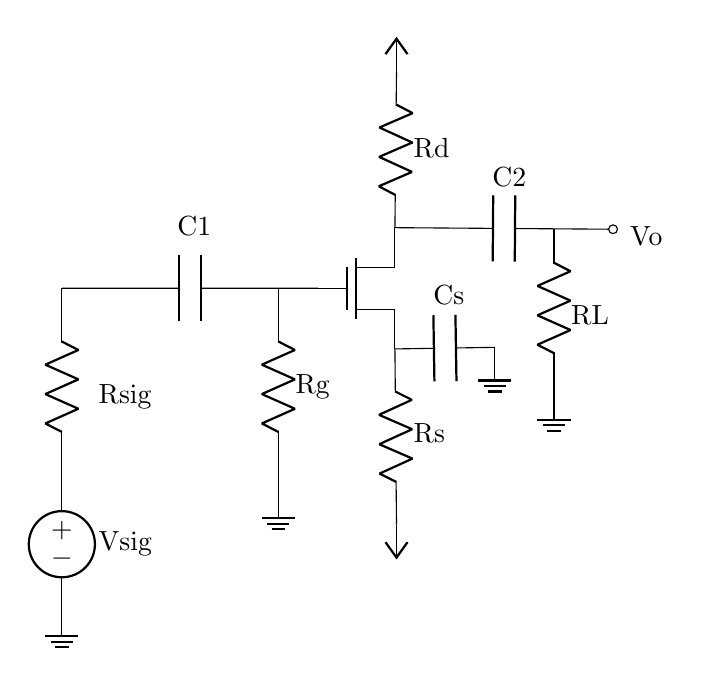
\begin{tikzpicture}
	% Paths, nodes and wires:
	\node[nmos] at (9.48, 7){};
	\draw (8.5, 7) to[capacitor] (5.25, 7);
	\draw (9.48, 6.23) to[capacitor] (10.75, 6.25);
	\draw (9.48, 7.77) to[capacitor] (12.25, 7.75);
	\draw (5.25, 7) to[american resistor] (5.25, 4.5);
	\draw (8, 7) to[american resistor] (8, 4.5);
	\draw (9.48, 6.23) to[american resistor] (9.5, 4);
	\draw (11.5, 7.75) to[american resistor] (11.5, 5.75);
	\draw (9.48, 7.77) to[american resistor] (9.5, 9.75);
	\node[ground] at (8, 4.5){};
	\node[ground] at (10.75, 6.25){};
	\node[ground] at (11.5, 5.75){};
	\node[vee] at (9.5, 4){};
	\node[vcc] at (9.5, 9.75){};
	\draw (5.25, 4.5) to[american voltage source] (5.25, 3);
	\node[ground] at (5.25, 3){};
	\node[ocirc] at (12.25, 7.75){};
	\node[shape=rectangle, minimum width=0.965cm, minimum height=0.715cm] at (6, 5.625){} node[anchor=north west, align=left, text width=0.577cm, inner sep=6pt] at (5.5, 6){Rsig};
	\node[shape=rectangle, minimum width=0.965cm, minimum height=0.715cm] at (6, 3.75){} node[anchor=north west, align=left, text width=0.577cm, inner sep=6pt] at (5.5, 4.125){Vsig};
	\node[shape=rectangle, minimum width=0.965cm, minimum height=0.715cm] at (7, 7.75){} node[anchor=north west, align=left, text width=0.577cm, inner sep=6pt] at (6.5, 8.125){C1};
	\node[shape=rectangle, minimum width=0.965cm, minimum height=0.715cm] at (10.25, 6.875){} node[anchor=north west, align=left, text width=0.577cm, inner sep=6pt] at (9.75, 7.25){Cs};
	\node[shape=rectangle, minimum width=0.965cm, minimum height=0.715cm] at (11, 8.375){} node[anchor=north west, align=left, text width=0.577cm, inner sep=6pt] at (10.5, 8.75){C2};
	\node[shape=rectangle, minimum width=0.965cm, minimum height=0.715cm] at (8.5, 5.75){} node[anchor=north west, align=left, text width=0.577cm, inner sep=6pt] at (8, 6.125){Rg};
	\node[shape=rectangle, minimum width=0.965cm, minimum height=0.715cm] at (10, 5.125){} node[anchor=north west, align=left, text width=0.577cm, inner sep=6pt] at (9.5, 5.5){Rs};
	\node[shape=rectangle, minimum width=0.965cm, minimum height=0.715cm] at (12, 6.625){} node[anchor=north west, align=left, text width=0.577cm, inner sep=6pt] at (11.5, 7){RL};
	\node[shape=rectangle, minimum width=0.965cm, minimum height=0.715cm] at (10, 8.75){} node[anchor=north west, align=left, text width=0.577cm, inner sep=6pt] at (9.5, 9.125){Rd};
	\node[shape=rectangle, minimum width=0.965cm, minimum height=0.715cm] at (12.75, 7.625){} node[anchor=north west, align=left, text width=0.577cm, inner sep=6pt] at (12.25, 8){Vo};
\end{tikzpicture}
  \caption{Full Schematic of the Common-Source Amplifier}
  \label{fig:full_circuit}
\end{figure}

\paragraph{Part 1: Design and Simulation}
First, a DC and AC analysis was performed by hand to design the amplifier. The design goals were $I_D = \SI{1}{mA}$ and $A_v \le \SI{-5}{V/V}$, using given transistor parameters ($k_n$, $V_{tn}$, $\lambda$). This analysis determined the required values for the source resistor $R_S$ and drain resistor $R_D$.

The circuit was then simulated in LTspice using the calculated resistor values and the provided 2N7000 SPICE model. A $20 \text{ mV}_{\text{pk-pk}}$, $1 \text{ kHz}$ sinusoidal input signal ($v_{sig}$) was applied. The simulation was used to measure the DC operating point ($V_{GS}, V_{DS}, I_D$) and the AC voltage gain $A_v$, which were then compared to the hand calculations.

\paragraph{Part 2: Prototyping}
The circuit was assembled on a breadboard using standard resistor values close to the calculated design values, as shown in Figure \ref{fig:breadboard}.

\begin{figure}[H]
  \centering
  \includegraphics[width=0.5\textwidth]{Circuit.png}
  \caption{The prototyped NMOS CS amplifier circuit on the breadboard.}
  \label{fig:breadboard}
\end{figure}

\paragraph{Part 3: Measurements}
Several measurements were taken from the prototyped circuit.
\begin{itemize}
  \item \textbf{DC Bias Point:} A digital multimeter was used to measure the DC voltages at the gate ($V_G$), source ($V_S$), and drain ($V_D$). All resistor values were also measured.
  \item \textbf{AC Voltage Gain:} A function generator applied a $20 \text{ mV}_{\text{pk-pk}}$, $1 \text{ kHz}$ sinusoid, and an oscilloscope was used to measure the AC output ($v_o$) and input ($v_{sig}$) waveforms to determine the gain $A_v$.
  \item \textbf{Output Resistance:} The load resistor $R_L$ was replaced with a $\SI{1}{M\ohm}$ resistor and the output amplitude was measured. $R_L$ was then adjusted (using a $4.7 \text{ k}\Omega$ resistor) until the output amplitude was approximately 50\% of this "open-load" value. This value of $R_L$ is equal to the output resistance $R_o$.
\end{itemize}
Finally, post-measurement calculations were performed to find the experimental $I_D$, $A_v$, and $R_o$, and all three sets of results (hand-calculated, simulated, and measured) were compared.

% --- RESULTS AND CONCLUSIONS (DISCUSSION) ---
\section{Results and Conclusions (Discussion)}

\subsection{Hand Calculations (Design)}

\subsubsection{DC Operating Point Analysis}
\paragraph{Given Parameters}
\begin{itemize}
  \item \textbf{Voltage Supplies:} $V_{+} = \SI{15}{\volt}$, $V_{-} = \SI{-15}{\volt}$
  \item \textbf{Design Goals:} $I_{D} = \SI{1}{\milli\ampere}$, $A_{v} \le \SI{-5}{\volt/\volt}$
  \item \textbf{Circuit Resistors:} $R_{sig} = \SI{50}{\ohm}$, $R_{L} = \SI{10}{\kilo\ohm}$, $R_{G} = \SI{10}{\kilo\ohm}$
  \item \textbf{Transistor Parameters (2N7000):} $\lambda = \SI{0.0146}{\per\volt}$, $k_{n} = \SI{1.08}{\milli\ampere\per\volt\squared}$, $V_{tn} = \SI{1.45}{\volt}$
\end{itemize}

\begin{figure}[H]
  \centering
  \begin{circuitikz}[scale=1.2]
    % Define power rails
    \node[vcc](Vcc) at (0, 5) {$V_+ = \SI{15}{\volt}$};
    \node[vee](Vee) at (0, -5) {$V_- = \SI{-15}{\volt}$};

    % Transistor
    \node[nmos, anchor=S](Q1) at (0, 0) {};

    % Resistors
    \draw (Q1.D) to[R, l_=$R_D$] (Q1.D |- Vcc.south) -- (Vcc);
    \draw (Q1.S) to[R, l_=$R_S$] (Q1.S |- Vee.north) -- (Vee);
    \draw (Q1.G) to[R, l=$R_G$] ++(-2.5,0) node[ground](GND){};

    % Capacitors (open) - repositioned for better spacing
    \draw (Q1.G) ++(-5,0) to[C, l=$C_{C1}$, o-o] ++(2,0);
    \draw (Q1.D) to[C, l=$C_{C2}$, o-o] ++(2.5,0);
    \draw (Q1.S) to[C, l_=$C_S$, o-o] ++(2.5,0);

    % Labels for nodes - repositioned to avoid overlap
    \draw (Q1.G) node[above left, xshift=-1mm, yshift=1mm] {$V_G$};
    \draw (Q1.D) node[above right, xshift=1mm, yshift=1mm] {$V_D$};
    \draw (Q1.S) node[below right, xshift=1mm, yshift=-1mm] {$V_S$};
  \end{circuitikz}
  \caption{DC Model of the Common-Source Amplifier}
  \label{fig:dc_model}
\end{figure}

\paragraph{1. DC Gate Current and Voltage ($I_G$, $V_G$)}
The DC gate current $I_G$ for a MOSFET is effectively $\SI{0}{\ampere}$. Assuming $R_G$ connects the gate to ground, the DC voltage drop is $I_G \cdot R_G = \SI{0}{\volt}$.
Therefore, the DC gate voltage is $V_G = \SI{0}{\volt}$.

\paragraph{2. Overdrive Voltage ($V_{OV}$)}
Using the saturation current equation for the design goal $I_D = \SI{1}{\milli\ampere}$:
$$
I_D = \frac{1}{2} k_n (V_{OV})^2
$$
$$
\SI{1}{\milli\ampere} = \frac{1}{2} (\SI{1.08}{\milli\ampere\per\volt\squared}) (V_{OV})^2
$$
$$
V_{OV}^2 = \frac{\SI{2}{\milli\ampere}}{\SI{1.08}{\milli\ampere\per\volt\squared}} \approx \SI{1.8519}{\volt\squared}
$$
$$
V_{OV} = \sqrt{\SI{1.8519}{\volt\squared}} \approx \SI{1.361}{\volt}
$$

\paragraph{3. Transconductance ($g_m$) and Gate-Source Voltage ($V_{GS}$)}
$$
g_m = \frac{2 I_D}{V_{OV}} = \frac{2 \cdot \SI{1}{\milli\ampere}}{\SI{1.361}{\volt}} \approx \SI{1.4695}{\milli\ampere\per\volt} \text{ (or \SI{1.47}{\milli S})}
$$
$$
V_{GS} = V_{OV} + V_{tn} = \SI{1.361}{\volt} + \SI{1.45}{\volt} = \SI{2.811}{\volt}
$$

\paragraph{4. Early Effect Resistance ($r_o$)}
$$
r_o = \frac{1}{\lambda I_D} = \frac{1}{(\SI{0.0146}{\per\volt}) (\SI{1}{\milli\ampere})} \approx \SI{68.5}{\kilo\ohm}
$$

\paragraph{5. Source Resistor ($R_S$)}
First, find the DC source voltage $V_S$ using $V_G = \SI{0}{\volt}$:
$$
V_{GS} = V_G - V_S \implies \SI{2.811}{\volt} = \SI{0}{\volt} - V_S \implies V_S = \SI{-2.811}{\volt}
$$
$R_S$ connects the source terminal ($V_S$) to the negative supply ($V_- = \SI{-15}{\volt}$). The DC current through it is $I_S = I_D = \SI{1}{\milli\ampere}$.
$$
R_S = \frac{V_S - V_{-}}{I_D} = \frac{\SI{-2.811}{\volt} - (\SI{-15}{\volt})}{\SI{1}{\milli\ampere}} = \frac{\SI{12.189}{\volt}}{\SI{1}{\milli\ampere}} = \SI{12.19}{\kilo\ohm}
$$
A standard $\SI{12.1}{\kilo\ohm}$ resistor will be used.

\subsubsection{AC Analysis}

\begin{figure}[H]
  \centering
  \begin{circuitikz}[scale=1.1, transform shape]
    % Input side
    \draw (0,0) to[sV, l=$v_{sig}$] (0,2.5) to[R, l=$R_{sig}$] (2.5,2.5)
    coordinate (Vin) to[short] (4,2.5) coordinate (Vi)
    node[above right, xshift=1mm] {$v_i$};

    % Gate resistor
    \draw (Vi) to[R, l_=$R_G$, *-] (4,0) node[ground](GND){};

    % Small-signal model
    \draw (Vi) -- (5.5,2.5) node[above, yshift=1mm]{G}; % Gate
    \draw (5.5,0) node[ground]{} -- (5.5,0) node[below, yshift=-1mm]{S}; % Source

    % Dependent current source
    \draw (8,3) to[cI, l=$g_m v_{gs}$] (8,0);

    % Input voltage v_gs - moved further right
    \draw [dashed] (5.5,2.5) -- (5.5,0);
    \draw [<->] (6.2, 2.5) -- (6.2, 0) node [midway, right] {$v_{gs} = v_i$};

    % Output side
    \draw (8,3) -- (11,3) coordinate (Vo) node[above right, xshift=1mm] {$v_o$};
    \draw (8,0) -- (14,0) node[ground]{};

    % Output resistors - better spacing
    \draw (Vo) to[R, l_=$r_o$, *-] (11,0);
    \draw (Vo) to[short] (12.5,3) to[R, l=$R_D$] (12.5,0);
    \draw (Vo) to[short] (14,3) to[R, l=$R_L$] (14,0);
  \end{circuitikz}
  \caption{AC Small-Signal Model of the Common-Source Amplifier}
  \label{fig:ac_model}
\end{figure}

\paragraph{1. Input Voltage Ratio ($v_i / v_{sig}$)}
The AC input resistance is $R_{in} = R_G = \SI{10}{\kilo\ohm}$.
$$
\frac{v_i}{v_{sig}} = \frac{R_G}{R_{sig} + R_G} = \frac{\SI{10000}{\ohm}}{\SI{50}{\ohm} + \SI{10000}{\ohm}} \approx 0.995
$$
(We will approximate $v_i \approx v_{sig}$).

\paragraph{2. Drain Resistor ($R_D$) for Gain $A_v = -5$ V/V}
The AC bypass capacitor $C_S$ shorts $R_S$ to ground. The gain is:
$$
A_v = -g_m (r_o \parallel R_D \parallel R_L)
$$
Solving for $R_D$ to get $A_v = \SI{-5}{\volt/\volt}$:
$$
\SI{-5}{\volt/\volt} = -(\SI{1.4695}{\milli S}) ( \SI{68.5}{\kilo\ohm} \parallel R_D \parallel \SI{10}{\kilo\ohm} )
$$
Let $R_{L}' = r_o \parallel R_L = \SI{68.5}{\kilo\ohm} \parallel \SI{10}{\kilo\ohm} \approx \SI{8.726}{\kilo\ohm}$.
$$
5 = (\SI{1.4695}{\milli S}) ( R_D \parallel \SI{8.726}{\kilo\ohm} )
$$
Let $R_{eq} = R_D \parallel \SI{8.726}{\kilo\ohm}$.
$$
R_{eq} = \frac{5}{\SI{1.4695}{\milli S}} \approx \SI{3.4025}{\kilo\ohm}
$$
Now, solve for $R_D$:
$$
\frac{1}{R_D} = \frac{1}{R_{eq}} - \frac{1}{R_{L}'} = \frac{1}{\SI{3.4025}{\kilo\ohm}} - \frac{1}{\SI{8.726}{\kilo\ohm}} \approx \SI{0.1793}{\milli S}
$$
$$
R_D = \frac{1}{\SI{0.1793}{\milli S}} \approx \SI{5.577}{\kilo\ohm}
$$
A standard $\SI{5.6}{\kilo\ohm}$ resistor will be used.

\paragraph{3. DC Drain Voltage ($V_D$) and Saturation Check}
Using $R_D = \SI{5.577}{\kilo\ohm}$:
$$
V_D = V_{+} - I_D R_D = \SI{15}{\volt} - (\SI{1}{\milli\ampere})(\SI{5.577}{\kilo\ohm}) = \SI{9.423}{\volt}
$$
Check saturation condition: $V_{DS} \ge V_{OV}$.
$$
V_{DS} = V_D - V_S = \SI{9.423}{\volt} - (\SI{-2.811}{\volt}) = \SI{12.234}{\volt}
$$
Since $V_{DS} (\SI{12.234}{\volt}) \ge V_{OV} (\SI{1.361}{\volt})$, the transistor is in saturation.

\paragraph{4. Amplifier Output Resistance ($R_o$)}
The output resistance $R_o$ is $R_D$ in parallel with $r_o$.
$$
R_o = R_D \parallel r_o = \SI{5.577}{\kilo\ohm} \parallel \SI{68.5}{\kilo\ohm} \approx \SI{5.157}{\kilo\ohm}
$$

\subsection{Simulation Results}
\begin{table}[H]
  \centering
  \caption{Simulation Results}
  \label{tab:sim_results}
  \sisetup{round-mode=places,round-precision=3}
  \begin{tabular}{lc}
    \toprule
    \textbf{Parameter} & \textbf{Simulated Value} \\
    \midrule
    $V_G$ & \SI{0}{\volt} \\
    $V_D$ & \SI{9.314}{\volt} \\
    $V_S$ & \SI{-2.715}{\volt} \\
    $V_{GS}$ & \SI{2.715}{\volt} \\
    $V_{DS}$ & \SI{12.029}{\volt} \\
    $I_D$ & \SI{1.015}{\milli\ampere} \\
    $A_v = v_o / v_i$ & \SI{-5.487}{\volt/\volt} \\
    \bottomrule
  \end{tabular}
\end{table}

\subsection{Measurement Data}
\begin{table}[H]
  \centering
  \caption{Measured Component Values}
  \label{tab:measured_components}
  \sisetup{round-mode=places,round-precision=3}
  \begin{tabular}{lc}
    \toprule
    \textbf{Component} & \textbf{Measured Value} \\
    \midrule
    $R_D$ ($\SI{5.6}{\kilo\ohm}$ nominal) & \SI{5.65}{\kilo\ohm} \\
    $R_S$ ($\SI{12.1}{\kilo\ohm}$ nominal) & \SI{12.11}{\kilo\ohm} \\
    $R_G$ ($\SI{10}{\kilo\ohm}$ nominal) & \SI{9.67}{\kilo\ohm} \\
    $R_L$ ($\SI{10}{\kilo\ohm}$ nominal) & \SI{9.4}{\kilo\ohm} \\
    $R_{sig}$ ($\SI{50}{\ohm}$ nominal) & \SI{46.1}{\ohm} \\
    \bottomrule
  \end{tabular}
\end{table}

\begin{table}[H]
  \centering
  \caption{Measured DC and AC Values}
  \label{tab:measured_dc_ac}
  \sisetup{round-mode=places,round-precision=3}
  \begin{tabular}{lc}
    \toprule
    \textbf{Parameter} & \textbf{Measured Value} \\
    \midrule
    $V_G$ & \SI{0}{\volt} \\
    $V_D$ & \SI{7.54}{\volt} \\
    $V_S$ & \SI{-2.256}{\volt} \\
    $v_{sig}$ (pk-pk) & \SI{20.8}{\milli\volt} \\
    $v_o$ (pk-pk, $R_L=\SI{9.4}{\kilo\ohm}$) & \SI{68}{\milli\volt} \\
    $R_o$ (from 50\% amplitude) & $\approx \SI{4.7}{\kilo\ohm}$ \\
    \bottomrule
  \end{tabular}
\end{table}

\begin{figure}[H]
  \centering
  \includegraphics[width=0.9\textwidth]{10k_resistor_measurements.png}
  \caption{Oscilloscope reading for AC gain ($A_v$) with $R_L = \SI{9.4}{\kilo\ohm}$. Ch1 (Yellow): $v_{sig} = \SI{20.8}{mV_{pk-pk}}$. Ch2 (Blue): $v_o = \SI{68}{mV_{pk-pk}}$.}
  \label{fig:ac_gain_measurement}
\end{figure}

\begin{figure}[H]
  \centering
  \begin{subfigure}{0.48\textwidth}
    \includegraphics[width=\textwidth]{1M_resistor_measurements.png}
    \caption{"Open-load" ($R_L \approx \SI{1}{M\ohm}$) output $v_o \approx \SI{104}{mV_{pk-pk}}$.}
    \label{fig:ro_open}
  \end{subfigure}
  \hfill
  \begin{subfigure}{0.48\textwidth}
    \includegraphics[width=\textwidth]{4_7k_resistor_measurements.png}
    \caption{Output with $R_L = \SI{4.7}{k\ohm}$. $v_o \approx \SI{52}{mV_{pk-pk}}$, which is 50\% of the open-load voltage.}
    \label{fig:ro_loaded}
  \end{subfigure}
  \caption{Oscilloscope measurements for determining the output resistance $R_o$.}
  \label{fig:ro_measurement}
\end{figure}

\paragraph{Post-Measurement Calculations}
Using measured values from Tables \ref{tab:measured_components} and \ref{tab:measured_dc_ac}, and measured $V_+ = \SI{15.036}{\volt}$ and $V_- = \SI{-15.079}{\volt}$:
$$
V_{GS} = V_G - V_S = \SI{0}{\volt} - (\SI{-2.256}{\volt}) = \SI{2.256}{\volt}
$$
$$
V_{DS} = V_D - V_S = \SI{7.54}{\volt} - (\SI{-2.256}{\volt}) = \SI{9.796}{\volt}
$$
$$
I_D = \frac{V_S - V_{-}}{R_S} = \frac{\SI{-2.256}{\volt} - (\SI{-15.079}{\volt})}{\SI{12.11}{\kilo\ohm}} = \frac{\SI{12.823}{\volt}}{\SI{12110}{\ohm}} = \SI{1.059}{\milli\ampere}
$$
Calculate $v_i$ from measured $v_{sig}$:
$$
v_i = v_{sig} \frac{R_G}{R_{sig} + R_G} = \SI{20.8}{\milli\volt} \frac{\SI{9.67}{\kilo\ohm}}{\SI{46.1}{\ohm} + \SI{9.67}{\kilo\ohm}} = \SI{20.70}{\milli\volt}
$$
$$
A_v = v_o / v_i = \frac{-\SI{68}{\milli\volt}}{\SI{20.70}{\milli\volt}} = \SI{-3.285}{\volt/\volt}
$$
$$
R_o = \text{Value from Table \ref{tab:measured_dc_ac}} \approx \SI{4.7}{\kilo\ohm}
$$

\subsection{Comparison of Results}
\begin{table}[H]
  \centering
  \caption{Comparison of Calculated, Simulated, and Measured Values}
  \label{tab:final_compare}
  \sisetup{round-mode=places,round-precision=3}
  \begin{tabular}{lccc}
    \toprule
    \textbf{Parameter} & \textbf{Hand Calc (Goal)} & \textbf{Simulation} & \textbf{Measured} \\
    \midrule
    $V_{GS}$ & \SI{2.811}{\volt} & \SI{2.715}{\volt} & \SI{2.256}{\volt} \\
    $V_{DS}$ & \SI{12.234}{\volt} & \SI{12.029}{\volt} & \SI{9.796}{\volt} \\
    $I_D$ & \SI{1.0}{\milli\ampere} & \SI{1.015}{\milli\ampere} & \SI{1.059}{\milli\ampere} \\
    $A_v$ & \SI{-5.0}{\volt/\volt} & \SI{-5.487}{\volt/\volt} & \SI{-3.285}{\volt/\volt} \\
    $R_o$ & \SI{5.157}{\kilo\ohm} & (N/A) & \SI{4.7}{\kilo\ohm} \\
    \bottomrule
  \end{tabular}
\end{table}

\subsection{Discussion}
The results from the hand calculations and the LTspice simulation show excellent agreement. The simulated $I_D$ of $\SI{1.015}{mA}$ was within 1.5\% of the $\SI{1.0}{mA}$ design goal, and the simulated gain $A_v = \SI{-5.487}{V/V}$ was very close to the target of $\SI{-5.0}{V/V}$. This validates the design equations and the simulation model.

Comparing the measured results to the calculated and simulated values reveals several discrepancies, which can be explained by variations in the physical transistor parameters.
\begin{itemize}
  \item \textbf{DC Operating Point:} The measured $I_D$ ($\SI{1.059}{mA}$) was very close to the design goal ($\SI{1.0}{mA}$). However, the measured $V_{GS}$ ($\SI{2.256}{V}$) was significantly *lower* than the calculated ($\SI{2.811}{V}$) and simulated ($\SI{2.715}{V}$) values. As noted in the lab manual, the most likely cause is that the threshold voltage ($V_{tn}$) of the specific 2N7000 transistor used was lower than the $\SI{1.45}{V}$ value from the datasheet used in the calculations. A lower $V_{tn}$ would require a smaller $V_{GS}$ to achieve the same $I_D$.

  \item \textbf{Voltage Gain ($A_v$):} The measured gain $A_v = \SI{-3.285}{V/V}$, supported by the data in Figure \ref{fig:ac_gain_measurement}, was substantially lower than the calculated goal ($\SI{-5.0}{V/V}$) and the simulation ($\SI{-5.487}{V/V}$). The gain is given by $A_v = -g_m (R_{eq})$, where $R_{eq} = R_D \parallel r_o \parallel R_L$. The measured $R_{eq}$ (using measured component values) is $\approx \SI{3.42}{k\Omega}$, which is very close to the design value. This implies that the discrepancy must come from the transconductance, $g_m$.

    The measured $g_m$ can be estimated as $|A_v| / R_{eq} = 3.285 / \SI{3.42}{k\Omega} \approx \SI{0.96}{mS}$. This is much lower than the calculated $g_m = \SI{1.47}{mS}$. Since $g_m = \sqrt{2 k_n I_D}$ and the measured $I_D$ was accurate, this strongly suggests that the actual process transconductance parameter ($k_n$) of the transistor was significantly lower than the $1.08 \text{ mA/V}^2$ value used in the design.

  \item \textbf{Output Resistance ($R_o$):} The measured output resistance was $R_o \approx \SI{4.7}{k\Omega}$. This was determined by finding the load $R_L$ that caused the output amplitude to drop to 50\% of its "open-load" value, as shown in Figure \ref{fig:ro_measurement}. This result is in good agreement with the calculated value of $R_o = R_D \parallel r_o = \SI{5.157}{k\Omega}$. A theoretical $R_o$ based on measured component values ($R_D = \SI{5.65}{k\Omega}$ and $r_o \approx \SI{64.7}{k\Omega}$) would be $\SI{5.19}{k\Omega}$. The measured value is close to this and correctly follows the hint $R_o \le R_D$ ($\SI{4.7}{k\Omega} \le \SI{5.65}{k\Omega}$).

  \item \textbf{Further Exploration:} When the input signal amplitude was increased to $\SI{1}{V_{pk-pk}}$, the output waveform began to show significant distortion (clipping), as seen in Figure \ref{fig:distortion}. This occurs because the large-signal $v_{gs}$ violates the small-signal condition ($v_{gs} \ll 2V_{OV}$) and pushes the transistor out of the saturation region (into cutoff or triode), which is required for linear amplification.
\end{itemize}

\begin{figure}[H]
  \centering
  \includegraphics[width=0.9\textwidth]{1vinput.png}
  \caption{Output signal distortion (clipping) when the input signal $v_{sig}$ was increased to $\approx \SI{1}{V_{pk-pk}}$.}
  \label{fig:distortion}
\end{figure}

\subsection{Conclusion}
This lab successfully demonstrated the design, simulation, and implementation of an NMOS common-source amplifier. The design goals were closely met in simulation, but the physical prototype showed deviations in performance. The measured gain ($A_v = \SI{-3.285}{V/V}$) was lower than the $\SI{-5.0}{V/V}$ target, while the DC bias current ($I_D = \SI{1.059}{mA}$) was very accurate.

The discrepancies between theory and measurement are primarily attributed to the inherent variations in the 2N7000 transistor's physical parameters, specifically a lower-than-assumed $V_{tn}$ and $k_n$. The measured output resistance $R_o \approx \SI{4.7}{k\Omega}$ showed good agreement with the theoretical value. This exercise successfully highlighted the core principles of CS amplifier operation and the significant impact of real-world component tolerances on circuit performance.

% --- BIBLIOGRAPHY ---
\section{Bibliography}
[1] Fixel, Debora. "ENGR 305 - Lab 9: NMOS Common-Source Amplifier." Trinity College, Hartford, CT, October 2025.
\newline

[2] Microchip Technology Inc. "2N7000 N-Channel Enhancement-Mode Vertical DMOS FET." Datasheet, DS20005695A, 2021.
\end{document}
